\documentclass[spanish,a4paper,11pt,twoside]{report}
%%%%%%%%%%%%%%%%%%%%%%%%%%%%%%%%%%%%%%%%%%%%%%%%%%%%%%%%%%%%%%%%%%%%%%%%%%%%%%%
\usepackage[utf8]{inputenc}
\usepackage[spanish]{babel}
\usepackage[dvips]{graphicx}
\usepackage[dvips]{epsfig}
\usepackage{alltt}
\usepackage{templates/algorithm}
\usepackage{templates/algorithmic}
\usepackage{templates/multirow}

%%%%%%%%%%%%%%%%%%%%%%%%%%%%%%%%%%%%%%%%%%%%%%%%%%%%%%%%%%%%%%%%%%%%%%%%%%%%%%%

\newcommand{\SONY}{{\sc Sony}}
\newcommand{\MICROSOFT}{{\sc Microsoft}}
\newcommand{\GCC}{\textsf{\textsc{G}CC}}
\newcommand{\INTEL}{\textsf{\textsc{I}ntel}}

%%% Traducimos el pseudocodigo
\renewcommand{\algorithmicwhile}{\textbf{mientras}}
\renewcommand{\algorithmicend}{\textbf{fin}}
\renewcommand{\algorithmicdo}{\textbf{hacer}}
\renewcommand{\algorithmicif}{\textbf{si}}
\renewcommand{\algorithmicthen}{\textbf{entonces}}
\renewcommand{\algorithmicrepeat}{\textbf{repetir}}
\renewcommand{\algorithmicuntil}{\textbf{hasta que}}
\renewcommand{\algorithmicelse}{\textbf{en otro caso}}
\renewcommand{\algorithmicfor}{\textbf{para}}

%\newcommand{\RETURN}{\textbf{retornar} }
\newcommand{\RET}{\STATE \textbf{retornar} }
\newcommand{\TO}{\textbf{hasta} }
\newcommand{\AND}{\textbf{y} }
\newcommand{\OR}{\textbf{o} }

%%%%%%%%%%%%%%%%% Creamos un entorno para listar código fuente %%%%%%%%%%%%%%%
\newenvironment{sourcecode}
{\begin{list}{}{\setlength{\leftmargin}{1em}}\item\scriptsize\bfseries}
{\end{list}}

\newenvironment{littlesourcecode}
{\begin{list}{}{\setlength{\leftmargin}{1em}}\item\tiny\bfseries}
{\end{list}}

\newenvironment{summary}
{\par\noindent\begin{center}\textbf{Abstract}\end{center}\begin{itshape}\par\noindent}
{\end{itshape}}

\newenvironment{keywords}
{\begin{list}{}{\setlength{\leftmargin}{1em}}\item[\hskip\labelsep \bfseries Keywords:]}
{\end{list}}

\newenvironment{palabrasClave}
{\begin{list}{}{\setlength{\leftmargin}{1em}}\item[\hskip\labelsep \bfseries Palabras clave:]}
{\end{list}}


%%%%%%%%%%%%%%%%%%%%%%%%%%%%%%%%%%%%%%%%%%%%%%%%%%%%%%%%%%%%%%%%%%%%%%%%%%%%%%%
% Format
\textwidth 15 cm
\input{amssym.def}
%%%%%%%%%%%%%%%%%%%%%%%%%%%%%%%%%%%%%%%%%%%%%%%%%%%%%%%%%%%%%%%%%%%%%%%%%%%%%%%

\begin{document}

\pagestyle{empty}
\thispagestyle{empty}

\begin{center}

\includegraphics[width=0.25\textwidth]{images/logotipo-secundario-ULL}
\end{center}


\begin{center}
        {\Huge Regla del Trapecio} \\[4.0mm] 
        {\Huge Integración} \\[3.0mm]
        {\Large Samanta Belén Lara Giannone\\
                Óscar Méndez Villavicencio\\
                Nuria Cecilia Martín Cruz} \\[5mm]
        {\Large \textit{Grupo $2B$}} \\[5mm]


        {\em Técnicas Experimentales. $1^{er}$ curso. $2^{do}$ semestre} \\[10mm]
        Lenguajes y Sistemas Informáticos \\[5mm]
        Facultad de Matemáticas \\[5mm]
        
        Universidad de La Laguna \\
\end{center}

\begin{center}
  La Laguna, \today 
\end{center}

%%%%%%%%%%%%%%%%%%%%%%%%%%%%%%%%%%%%%%%%%%%%%%%%%%%%%%%%%%%%%%%%%%%%%%%%%%%%%%%
\newpage{\pagestyle{empty}\cleardoublepage}

\pagestyle{myheadings} 
\markboth{Samanta Belén Lara Giannone\\
          Óscar Méndez Villavicencio\\
          Nuria Cecilia Martín Cruz}{Regla del Trapecio}

%%%%%%%%%%%%%%%%%%%%%%%%%%%%%%%%%%%%%%%%%%%%%%%%%%%%%%%%%%%%%%%%%%%%%%%%%%%%%%%

\renewcommand{\thepage}{\roman{page}}
\setcounter{page}{1}

%%%%%%%%%%%%%%%%%%%%%%%%%%%%%%%%%%%%%%%%%%%%%%%%%%%%%%%%%%%%%%%%%%%%%%%%%%%%%%%

\tableofcontents

%%%%%%%%%%%%%%%%%%%%%%%%%%%%%%%%%%%%%%%%%%%%%%%%%%%%%%%%%%%%%%%%%%%%%%%%%%%%%%%
\newpage{\pagestyle{empty}\cleardoublepage}

\listoffigures

%%%%%%%%%%%%%%%%%%%%%%%%%%%%%%%%%%%%%%%%%%%%%%%%%%%%%%%%%%%%%%%%%%%%%%%%%%%%%%%
\newpage{\pagestyle{empty}\cleardoublepage}

\listoftables

%%%%%%%%%%%%%%%%%%%%%%%%%%%%%%%%%%%%%%%%%%%%%%%%%%%%%%%%%%%%%%%%%%%%%%%%%%%%%%%
\newpage{\pagestyle{empty}\cleardoublepage}

%%%%%%%%%%%%%%%%%%%%%%%%%%%%%%%%%%%%%%%%%%%%%%%%%%%%%%%%%%%%%%%%%%%%%%%%%%%%%%%
%Numeracion a partir del capitulo I
\renewcommand{\thepage}{\arabic{page}}
\setcounter{page}{1}

\setlength{\parindent}{5mm}

%%%%%%%%%%%%%%%%%%%%%%%%%%%%%%%%%%%%%%%%%%%%%%%%%%%%%%%%%%%%%%%%%%%%%%%%%%%%%%%
\chapter{Motivación y objetivos}
\label{chapter:obj}
%%%%%%%%%%%%%%%%%%%%%%%%%%%%%%%%%%%%%%%%%%%%%%%%%%%%%%%%%%%%%%%%%%%%%%%%%%%%%
% Capítulo 1: Motivación y Objetivos 
%%%%%%%%%%%%%%%%%%%%%%%%%%%%%%%%%%%%%%%%%%%%%%%%%%%%%%%%%%%%%%%%%%%%%%%%%%%%%%%

%Los objetivos le dan al lector las razones por las que se realizó el
%proyecto o trabajo de investigación.

%---------------------------------------------------------------------------------
\section{Primera Seccióon}
\label{1:sec:1}
\parindent=0.5cm
\raggedright
El objetivo de este trabajo es realizar una integral mediante la Regla del Trapecio. La Regla
del Trapecio resulta de mucha utilidad dado que es una forma muy sencilla de aproximar el valor de
la integral definida entre dos puntos a y b. Geométricamente, es equivalente a aproximar el área del 
trapezoide bajo la línea recta que conecta f(a) y f(b).

%---------------------------------------------------------------------------------
\section{Segunda Sección}
\label{1:sec:2}
\parindent=0.5cm
\raggedright
Para la realización de este trabajo emplearemos la función:
$f(x)=\frac{1}{\sqrt(2\pi)} \quad\text{e}^{\frac{-x^2}{2}}$
comprendida en el itervalo [-1,1]


%%%%%%%%%%%%%%%%%%%%%%%%%%%%%%%%%%%%%%%%%%%%%%%%%%%%%%%%%%%%%%%%%%%%%%%%%%%%%%%
\chapter{Fundamentos teóricos}
\label{chapter:teo}
%%%%%%%%%%%%%%%%%%%%%%%%%%%%%%%%%%%%%%%%%%%%%%%%%%%%%%%%%%%%%%%%%%%%%%%%%%%%%%%
% Capítulo 2: Fundamentos Teóricos 
%%%%%%%%%%%%%%%%%%%%%%%%%%%%%%%%%%%%%%%%%%%%%%%%%%%%%%%%%%%%%%%%%%%%%%%%%%%%%%%

%++++++++++++++++++++++++++++++++++++++++++++++++++++++++++++++++++++++++++++++

%En este capítulo se han de presentar los antecedentes teóricos y prácticos que
%apoyan el tema objeto de la investigación.

%++++++++++++++++++++++++++++++++++++++++++++++++++++++++++++++++++++++++++++++
\section{Regla del Trapecio}
\label{2:sec:1}

Este método integración numérica calcula aproximadamente el valor de la integral definida. 
Se aproxima el valor de la integral de f(x) por el de la función lineal que pasa 
a través de los puntos(a,f(a)) y (b,f(b)). La integral de esta es igual al área del 
trapecio bajo la gráfica de la función lineal. Se sigue que: 
\[
\int_{a}^{b} f(x)dx \approx\left(b-a\right)\frac{f(a)+f(b)}{2} 
\]
Una estimación para el error de truncamiento local de una sola aplicación de la regla trapezoidal es:
\[
-\frac{\left(b-a\right)^3}{12}  \displaystyle f^{(2)}(\epsilon)
\]
Perteneciendo $\epsilon$ al intervalo entre a y b.


Una manera de mejorar la exactitud es utilizar la regla del trapecio compuesta, es decir, dividir
el intervalo de integración entre a y b en n subintervalos, cada uno de ancho
\[
\bigtriangleup{x}=\frac{b-a}{n}
\]
y aplicar el método a cada uno de ellos. Las ecuaciones resultantes son llamadas fórmulas
de integración de múltiple aplicación o compuestas.
\[
\int_{a}^{b} f(x)dx \sim\frac{h}{2}\left[f(a) + 2f(a+h) + 2f(a+2h) + ... + f(b)\right]
\]
Donde 
\[
h=\frac{b-a}{n} 
\]
La expresión anterior se puede escribir de la siguiente manera:
\[
\int_{a}^{b} f(x)dx \sim\frac{b-a}{n}\left(\frac{f(a)+f(b)}{2} + \sum_{k=1}^{n-1} a+k\frac{b-a}{n} \right)
\]


%%%%%%%%%%%%%%%%%%%%%%%%%%%%%%%%%%%%%%%%%%%%%%%%%%%%%%%%%%%%%%%%%%%%%%%%%%%%%%%
\chapter{Procedimiento experimental}
\label{chapter:exp}

%%%%%%%%%%%%%%%%%%%%%%%%%%%%%%%%%%%%%%%%%%%%%%%%%%%%%%%%%%%%%%%%%%%%%%%%%%%%%%%
% Capítulo 3: Procedimiento experimental 
%%%%%%%%%%%%%%%%%%%%%%%%%%%%%%%%%%%%%%%%%%%%%%%%%%%%%%%%%%%%%%%%%%%%%%%%%%%%%%%

%Este capítulo ha de contar con seccciones para la descripción de los experimentos 
%y del material.

%También debe haber una sección para los resultados obtenidos y una última de 
%análisis de los resultados.

%++++++++++++++++++++++++++++++++++++++++++++++++++++++++++++++++++++++++++++++
\section{Descripción de los experimentos}
\label{3:sec:1}
\parindent=0.5cm
\raggedright
\subsection{Primer experimento}
El experimento llevado a cabo es la realización de la integral definida, la aproximación
mediante la regla del trapecio y la regla del trapecio compuesta. Compararemos los resultados para ver si se obtiene una aproximacón fiable.
 Veamos\\
Integral definida 
\[
\int_{-1}^{1} \frac{1}{sqrt(2\pi)} \quad\text{e}^{\frac{-x^2}{2}}dx
\]
Regla del Trapecio
\[
\int_{-1}^{} \frac{1}{sqrt(2\pi)} \quad\text{e}^{\frac{-x^2}{2}}dx\approx\left(1-(-1)\right)\frac{f(-1)+f(1)}{2}
\]
Regla del Trapecio compuesta con n=4
\[
h=\frac{1-(-1)}{4} =\frac{1}{2} 
\]
\[
\int_{-1}^{1} \frac{1}{sqrt(2\pi)} \quad\text{e}^{\frac{-x^2}{2}}dx\approx\left[f(-1) + f(\frac-{1}{2}) + f(0) + f(\frac{1}{2} + f(1)\right]
\]


\subsection{Segundo experimento}
En este experimento vamos a ver los distintos errores que puede tomar el teorema para los posibles resultados de $\epsilon$.
Recordamos que $\epsilon$ pertenecerá al intervalo [a,b], en este caso, el intervalo [-1,1].
Por tanto,

\[
-\frac{\left(b-a\right)^3}{12}  \displaystyle f^{(2)}(\epsilon)
\]

para todo $\epsilon$ perteneciente al intervalo [-1,1].



%++++++++++++++++++++++++++++++++++++++++++++++++++++++++++++++++++++++++++++++
\section{Descripción del material}
\label{3:sec:2}
\parindent=0.2cm
\raggedright
El material que hemos empleado para la realización de este proyecto es el lenguaje de
programación Python, para la creación de los programas que verifican este método de integración, 
y el sistema de composición de textos \LaTeX para el diseño del proyecto.


%++++++++++++++++++++++++++++++++++++++++++++++++++++++++++++++++++++++++++++++
\section{Resultados obtenidos}
\label{3:sec:3}
\parindent=0.2cm
\raggedright
\subsection{Resultados del primer experimento}
Los resultados obtenidos son:
Integral definida 
\[
\int_{-1}^{1} \frac{1}{\sqrt(2\pi)} \quad\text{e}^{\frac{-x^2}{2}}dx\approx0.682689 
\]
Regla del Trapecio
\[
\int_{-1}^{1} \frac{1}{\sqrt(2\pi)} \quad\text{e}^{\frac{-x^2}{2}}dx\approx\left(1-(-1)\right)\frac{f(-1)+f(1)}{2}=0.483941
\]
Regla del Trapecio compuesta con n=4
\[
\int_{-1}^{1} \frac{1}{\sqrt(2\pi)} \quad\text{e}^{\frac{-x^2}{2}}dx\approx\left[f(-1) + f(\frac-{1}{2}) + f(0) + f(\frac{1}{2} + f(1)\right]\approx0.882385
\]
\subsection{resultados del segundo experimento}
Tomando varios valores de $\epsilon$,obtenemos la siguinte gráfica:








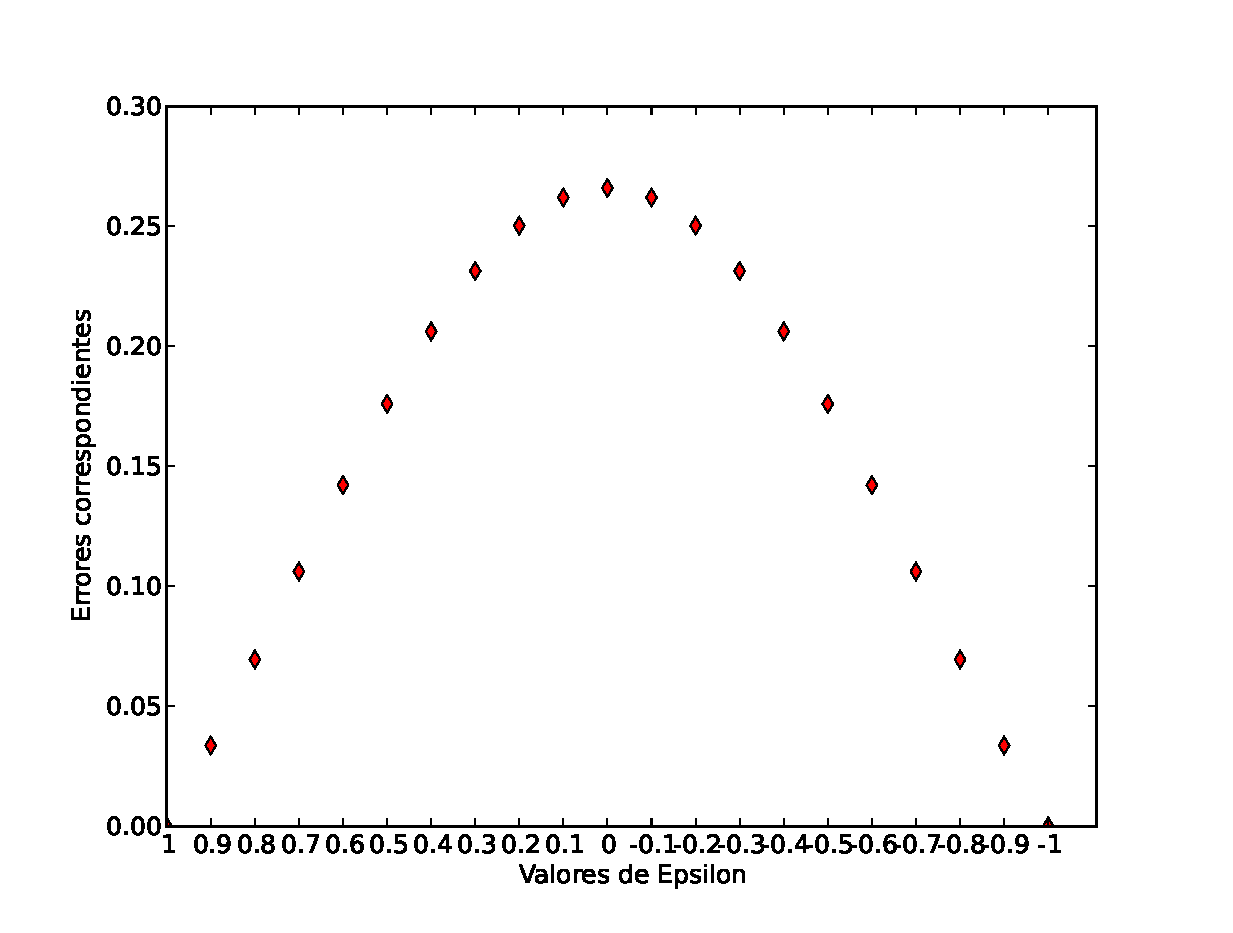
\includegraphics[width=1.25\textwidth]{images/imgraf}
%------------------------------------------------------------
%\begin{figure}[!th]
%\begin{center}
%\includegraphics[width=0.75\textwidth]{images/figura1.eps}
%\caption{Ejemplo de figura}
%\label{fig:1}
%\end{center}
%\end{figure}
%------------------------------------------------------------------------------
Resultados obtenidos en tiempo y velocidad para la regla del trapecio simple y la regla del trapecio compuesta
%--------------------------------------------------------------------------
\begin{table}[!ht]
\begin{center}
\begin{tabular}{|c|c|} \hline 
\textbf{Tiempo por Trapecio simple} & \textbf{Tiempo por trapecio compuesto} \\ 
\textbf{(en s)} & \textbf{(en s)} \\ \hline \hline
0.1412169 &
0.1414737
\\
\hline

0.1414649 &
0.1415798
\\
\hline

0.1412210 &
0.1413900
\\
\hline


\end{tabular}
\end{center}
\caption{Resultados experimentales de tiempo (s) y velocidad (m/s)}
\label{tab:1}
\end{table}


%------------------------------------------------------------------------------

%++++++++++++++++++++++++++++++++++++++++++++++++++++++++++++++++++++++++++++++
\section{Análisis de los resultados}
\label{3:sec:4}
\parindent=1cm
\raggedright
 


%%%%%%%%%%%%%%%%%%%%%%%%%%%%%%%%%%%%%%%%%%%%%%%%%%%%%%%%%%%%%%%%%%%%%%%%%%%%%%%
\chapter{Conclusiones}
\label{chapter:conclusiones}

%%%%%%%%%%%%%%%%%%%%%%%%%%%%%%%%%%%%%%%%%%%%%%%%%%%%%%%%%%%%%%%%%%%%%%%%%%%%%
% Capítulo 4: Conclusiones y Trabajos Futuros 
%%%%%%%%%%%%%%%%%%%%%%%%%%%%%%%%%%%%%%%%%%%%%%%%%%%%%%%%%%%%%%%%%%%%%%%%%%%%%%%

Podemos sacar muchas conclusiones de la aplicación de la integración por trapecio a esta función en particular.
Primeramente, cabe destacar que esta función es par, y por ello se simplifica mucho la operatoria a la hora de llevar a cabo todos los métodos.
En cuanmto a los análisis de los experimentos, nos dan información necesaria para sacar varias conclusiones. Como se esperaba, la integración por trapecio simple
es bastante más ineficiente que la integración por trapecio compuesta, ya que con sólo tomar cuatro divisiones del intervalo, ya se acerca bastante a la integral
definida .Por tanto, si escogemos un número de divisiones algo elevado, nuestra medida del área que se abarca va a ser aproximadamente acertada. 
Sin embargo, la integración por trapecio simple es un método que posee un error demasiado grande, que impide que nos podamos fiar de esta regla.
 No obstante, disponemos de una función que nos devuelve un error posible, y hemos comprobado que se cumple, en los experimentos llevados a cabo.
También la función del error es par, con lo que no era necesario tomar valores entre -1 y 1, sino que bastaba con tomarlos entre 0 y 1. Asimismo, igualando la
derivada de dicha función cero, pudimos obtener un error máximo, que es muy útil ya que el método del trapecio simple no es muy exacto. Con ello se consigue una cota 
superior e inferior de la integral definida, por lo que finalmente se le encuentra una gran utilidad a esta regla; debemos recordar que la regla del
trapecio compuesta no tiene un valor que nos pueda definir el error producido, ni por tanto ningún tipo de cota inferior o superior.

En el último experimento, vemos claramente que es más eficiente, en lo que se refiere la variable temporal, la regla del trapecio simple. Más aún si intentamos
precisar el resultado de la integral por el método compuesto, es decir, aumentar el número de divisiones del intervalo. Cuantas menos divisiones la diferencia de tiempos
y el porcentaje será menor. No obstante, está claro que el tiempo es influido no sólo por la complejidad del programa, puesto que en ocasiones, la regla compuesta
es más rápida que la regla simple de otro experimento, esto es, en estos casos la memoria y velocidad del ordenador se ven afectadas por otros procesos que 
puedan estar llevándose a cabo, con lo que el programa es más lento en esos momentos. Suponiendo un caso extremo, como un millón de divisiones, el programa sigue
funcionando, sin tardar en exceso (en ningún caso más de dos segundos, para poner un límite), y obtendríamos una aproximación muy exacta de la integral, y en esta
función en particular, el error que se obtendría no se podría notar ni siquiera en la diezmilésima, por lo que podemos afirmar que es un experimento muy eficiente si al 
menos nos permitimos un par de segundos. Si aumentamos más todavía el número de divisiones, el tiempo empleado iría creciendo exponencialmente puesto que le estaremos
exigiendo mucha potencia al ordenador, y no todos disponen de ella.


%%%%%%%%%%%%%%%%%%%%%%%%%%%%%%%%%%%%%%%%%%%%%%%%%%%%%%%%%%%%%%%%%%%%%%%%%%%%%%%

%%%%%%%%%%%%%%%%%%%%%%%%%%%%%%%%%%%%%%%%%%%%%%%%%%%%%%%%%%%%%%%%%%%%%%%%%%%%%%%
\newpage{\pagestyle{empty}\cleardoublepage}
\thispagestyle{empty}
\begin{appendix}

\chapter{Título del Apéndice 1}
\label{appendix:1}

\section{Algoritmo XXX}
\label{Apendice1:XXX}

\begin{center}
\begin{footnotesize}
\begin{verbatim}
###################################################################################
# Fichero .py
###################################################################################
#
# AUTORES
#   
# FECHA
#
# DESCRIPCION
#
###################################################################################
\end{verbatim}
\end{footnotesize}
\end{center}

\section{Algoritmo YYY}
\label{Apendice1:YYY}

\begin{center}
\begin{footnotesize}
\begin{verbatim}
/###################################################################################
 # Fichero .h
 ###################################################################################
 #
 # AUTORES
 #
 # FECHA
 #
 # DESCRIPCION
 #
 ##################################################################################
\end{verbatim}
\end{footnotesize}
\end{center}


\chapter{Título del Apéndice 2}
\label{appendix:2}

\section{Otro apéndice: Sección 1}
\label{Apéndice2:label}

\begin{center}
\begin{footnotesize}

\begin{verbatim}
Texto
\end{verbatim}

\end{footnotesize}
\end{center}

\section{Otro apéndice: Sección 2}
\label{Apéndice2:label2}

\begin{center}
\begin{footnotesize}

\begin{verbatim}
Texto
\end{verbatim}


\end{footnotesize}
\end{center}


\end{appendix}

%%%%%%%%%%%%%%%%%%%%%%%%%%%%%%%%%%%%%%%%%%%%%%%%%%%%%%%%%%%%%%%%%%%%%%%%%%%%%%%
\begin{bibliography}
\addcontentsline{toc}{chapter}{Bibliografía}
\bibliographystyle{plain}

\bibliography{bib/references}
\nocite{*}
\end{bibliography}

%%%%%%%%%%%%%%%%%%%%%%%%%%%%%%%%%%%%%%%%%%%%%%%%%%%%%%%%%%%%%%%%%%%%%%%%%%%%%%%


\end{document}
